\section{Results}
\label{sec:v2:results}
% GENERATED by scripts/real_results.py from repo files. Audit values are final; cost values are in progress (\prov).
\newcommand{\realAuditGemmaReported}{33.0}
\newcommand{\realAuditGemmaRecalc}{18.7}
\newcommand{\realAuditGptReported}{49.1}
\newcommand{\realAuditGptRecalc}{9.9}
\newcommand{\realAuditClaims}{40}
\newcommand{\realAuditReproduced}{31}
\newcommand{\realAuditContradicted}{2}
\newcommand{\realAuditNoArtifact}{7}
\newcommand{\realCostCalls}{\prov{122\,085}}
\newcommand{\realCostErrors}{\prov{655}}
\newcommand{\realCostLedgerMtok}{\prov{638}}
\newcommand{\realCostUsdLower}{\prov{84}}
\newcommand{\realCostWasteShare}{\prov{22}}
\newcommand{\realCostRitsShare}{\prov{96}}


Section~\ref{sec:v2:cmp} compares \capevolve{} with nine competitors and two controls at a matched checkpoint. Section~\ref{sec:v2:abl} ablates the surface, the orchestration mode and the gate on Suite D and on the main suites. Section~\ref{sec:v2:types} asks what each surface is worth, and Section~\ref{sec:v2:cost} reports cost, regressions and how often the gate says no. Red numbers with a dagger are placeholders and orange numbers are real but still change.
\needs{One sentence with the headline result, written only after the final evaluation.}

\subsection{Comparison at a matched checkpoint}
\label{sec:v2:cmp}

Every difference is paired with the seed artifact on the same tasks, intervals are family-cluster-robust, and p-values are Holm-adjusted inside their family (Section~\ref{sec:v2:stats}). Arms are compared at the matched checkpoint \ckpt{} (\mockBstarA{}, \mockBstarB{} and \mockBstarC{} target rollouts on Suites A, B and C). Table~\ref{tab:main_a} lists \capevolve{} with the stock gate (the shipped configuration), \capevolve{} with rule P, agent-optimize and the competitors against the seed on Suite A, where every arm edits the same two prompt files, so the comparison isolates the loop. The final set has \mockTA{} tasks scored once each for \mockSeedsA{} search seeds per arm, and the seed is scored twice.
\needs{How many arms beat the seed with Holm-adjusted $p<0.05$, which has the largest paired delta, and whether the CapEvolve configurations are above, level with (TOST) or below the best competitor.}

\begin{table*}[t]
\centering
\scriptsize
\setlength{\tabcolsep}{3.5pt}
\caption{Suite A results, baselines by ascending delta and CapEvolve last, with the exploratory stock-gate arm below. Score is the final-set reward. $\Delta$ is the paired difference in points with a family-cluster-robust 95\% interval, $p_{\mathrm{Holm}}$ is Holm-adjusted within the suite, and USD is optimizer cost at Sonnet list prices. Missing is missing over scheduled cells. Tokens and wall clock are in Table~\ref{tab:cost_tokens}, per-seed values in Table~\ref{tab:perseed}, promotions per search in Table~\ref{tab:promotions}. Suite A has no one-shot control. The stock-gate arm (E12A on Suite A, E12C on Suite C) is exploratory and outside the Holm family. (placeholder)}
\label{tab:main_a}
\begin{tabular}{lcccrrr}
\toprule
Arm & Score (\%) & $\Delta$ vs seed [CI] & $p_{\mathrm{Holm}}$ & USD & Missing \\
\midrule
\multicolumn{6}{l}{\textit{Suite A, SpreadsheetBench verified-400 (Gemma-4-31B-it)}} \\
\midrule
Seed (no search) & \pend{50.0} & ref. & -- & -- & \pend{0/140} \\
Meta-Harness & \pend{51.1} & \pend{+1.1 [$-$5.8, +8.0]} & \pend{1.000} & \pend{28} & \pend{0/210} \\
EvoSkill & \pend{52.2} & \pend{+2.2 [$-$4.6, +9.0]} & \pend{1.000} & \pend{17} & \pend{4/210} \\
GEPA & \pend{53.3} & \pend{+3.3 [$-$2.7, +9.4]} & \pend{1.000} & \pend{7} & \pend{5/210} \\
Trace2Skill & \pend{55.2} & \pend{+5.2 [$-$1.6, +12.0]} & \pend{0.687} & \pend{18} & \pend{0/210} \\
MIPROv2 & \pend{55.5} & \pend{+5.5 [$-$0.6, +11.6]} & \pend{0.496} & \pend{11} & \pend{1/210} \\
ACE & \pend{55.8} & \pend{+5.8 [+0.3, +11.3]} & \pend{0.290} & \pend{16} & \pend{5/210} \\
WikiSkill (community) & \pend{55.9} & \pend{+5.9 [$-$0.7, +12.5]} & \pend{0.496} & \pend{6} & \pend{1/210} \\
SkillOpt & \pend{56.7} & \pend{+6.7 [+0.3, +13.1]} & \pend{0.290} & \pend{10} & \pend{1/210} \\
CapEvolve HC & \pend{53.4} & \pend{+3.4 [$-$3.5, +10.3]} & \pend{1.000} & \pend{27} & \pend{5/210} \\
CapEvolve AO & \pend{53.6} & \pend{+3.6 [$-$3.4, +10.6]} & \pend{1.000} & \pend{36} & \pend{9/210} \\
CapEvolve HC, stock gate \textit{(exploratory)} & \pend{54.4} & \pend{+4.4 [$-$2.1, +10.9]} & -- & \pend{37} & \pend{8/210} \\
\bottomrule
\end{tabular}
\end{table*}


On Suites B and C the \capevolve{} arms edit prompt and tools while GEPA, MIPROv2 and ACE edit the prompt only, so a gap there mixes loop quality with surface width. Suite A and the prompt-only cells of Section~\ref{sec:v2:abl} separate the two. Suite B has \mockTB{} sealed test tasks scored \mockTrialsB{} times each and carries the one-shot control (Table~\ref{tab:main_bc}); Suite B has no stock-gate arm, so the shipped gate is not compared there. Suite C reuses the official airline test set of \mockTC{} tasks, which earlier work optimized against, so it is development-exposed and arms are not ranked on it.
\needs{Largest paired delta and number of arms below $p=0.05$ on each of Suites B and C, and whether the ordering agrees with Suite A.}

\begin{table*}[t]
\centering
\scriptsize
\setlength{\tabcolsep}{3.5pt}
\caption{Suites B and C results. Columns as in Table~\ref{tab:main_a}. (placeholder)}
\label{tab:main_bc}
\begin{tabular}{lcccrrr}
\toprule
Arm & Score (\%) & $\Delta$ vs seed [CI] & $\Delta$ vs one-shot [CI] & $p_{\mathrm{Holm}}$ in family & USD & Missing \\
\midrule
\multicolumn{7}{l}{\textit{Suite B, $\tau^2$ retail, sealed test-40 (gpt-oss-120b)}} \\
\midrule
\multicolumn{7}{l}{\textit{Reference arms}} \\
Seed (no search) & \pend{55.0} & ref. & \pend{$-$2.7} & -- & -- & \pend{2/120} \\
One-shot control & \pend{57.7} & \pend{+2.7 [$-$6.4, +11.7]} & ref. & \pend{1.000} & \pend{2} & \pend{5/360} \\
\multicolumn{7}{l}{\textit{Competitors, secondary family}} \\
GEPA & \pend{57.5} & \pend{+2.5 [$-$6.2, +11.2]} & \pend{$-$0.1 [$-$9.7, +9.6]} & \pend{1.000} & \pend{10} & \pend{6/360} \\
HarnessLens & \pend{61.6} & \pend{+6.6 [$-$0.5, +13.6]} & \pend{+3.9 [$-$3.9, +11.8]} & \pend{0.521} & \pend{15} & \pend{2/360} \\
\multicolumn{7}{l}{\textit{CapEvolve, primary family}} \\
CapEvolve HC & \pend{57.2} & \pend{+2.2 [$-$5.5, +9.8]} & \pend{+1.1 [$-$7.5, +9.6]} & \pend{1.000} & \pend{46} & \pend{9/360} \\
CapEvolve AO & \pend{55.3} & \pend{+0.3 [$-$7.7, +8.3]} & \pend{+0.6 [$-$8.3, +9.6]} & \pend{1.000} & \pend{33} & \pend{0/360} \\
\midrule
\multicolumn{7}{l}{\textit{Suite C, $\tau^2$ airline, official test-20 (development-exposed)}} \\
\midrule
\multicolumn{7}{l}{\textit{Reference arms}} \\
Seed (no search) & \pend{40.0} & ref. & \pend{+3.6} & -- & -- & \pend{2/60} \\
One-shot control & \pend{36.4} & \pend{$-$3.6 [$-$17.9, +10.8]} & ref. & \pend{1.000} & \pend{3} & \pend{2/180} \\
\multicolumn{7}{l}{\textit{Competitors, secondary family}} \\
HarnessLens & \pend{42.0} & \pend{+2.0 [$-$11.5, +15.4]} & \pend{+4.1 [$-$10.4, +18.6]} & \pend{1.000} & \pend{6} & \pend{0/180} \\
GEPA & \pend{44.1} & \pend{+4.1 [$-$6.6, +14.9]} & \pend{+8.9 [$-$2.7, +20.5]} & \pend{1.000} & \pend{13} & \pend{8/180} \\
\multicolumn{7}{l}{\textit{CapEvolve, primary family}} \\
CapEvolve HC & \pend{40.0} & \pend{+0.0 [$-$14.3, +14.3]} & \pend{+9.9 [$-$5.5, +25.3]} & \pend{1.000} & \pend{31} & \pend{3/180} \\
CapEvolve AO & \pend{43.9} & \pend{+3.9 [$-$9.9, +17.7]} & \pend{+9.2 [$-$5.7, +24.0]} & \pend{1.000} & \pend{16} & \pend{0/180} \\
\multicolumn{7}{l}{\textit{Exploratory, outside the Holm family}} \\
CapEvolve HC, stock gate & \pend{44.9} & \pend{+4.9 [$-$8.4, +18.2]} & \pend{+8.6 [$-$5.7, +23.0]} & -- & \pend{36} & \pend{1/180} \\
One-shot best of $k$ & \pend{44.5} & \pend{+4.5 [$-$7.1, +16.0]} & \pend{+8.0 [$-$4.5, +20.5]} & -- & \pend{23} & \pend{9/180} \\
\bottomrule
\end{tabular}
\end{table*}


\begin{figure*}[t]
\centering
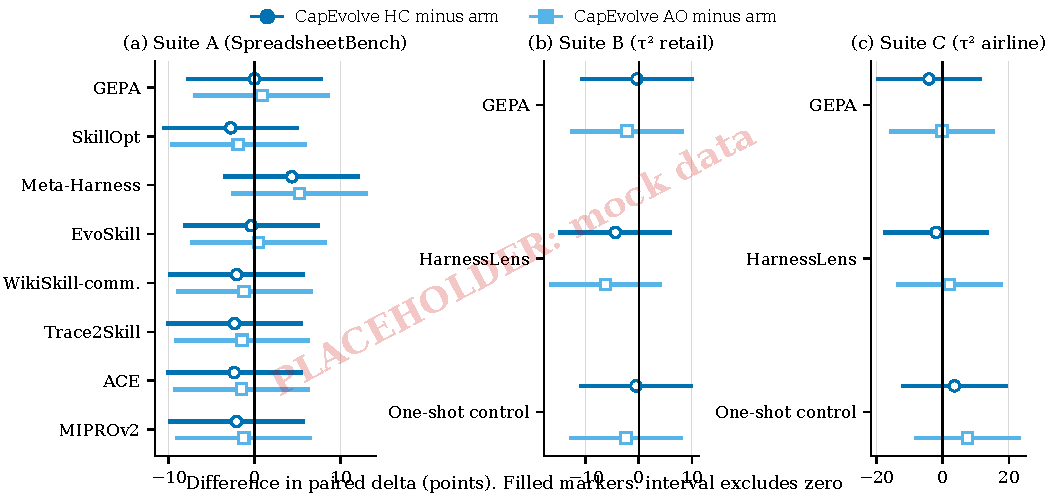
\includegraphics[width=\textwidth]{figures/fig_contrast.pdf}
\caption{Each \capevolve{} configuration against each competitor, as the difference in paired delta in points with 95\% intervals. Filled markers have intervals that exclude zero. These contrasts are the primary family (placeholder).}
\label{fig:contrast}
\end{figure*}

\subsection{Ablations}
\label{sec:v2:abl}

Each ablation changes one factor against the same reference cell and states the claim it tests, with a verdict in the pre-specified vocabulary: supported, equivalent, inconclusive or contradicted.

Surface width. Suite D holds the loop, the stock gate, the budget and the optimizer fixed and edits the prompt only, tools only, or both. The claim is that prompt and tools beats prompt only on tasks whose failures need deterministic enforcement. \needs{Suite D surface grid: paired gains of P, T and P+T over the seed, P+T against each single surface, the interaction term, both intervals, and the verdict. Do not write ``surface width matters'' unless the contrast exceeds the 10-point margin.}

Orchestration. Hill-climb and agent-optimize run on the main suites under rule P. The claim is that they reach equivalent final gain at matched rollouts and differ in cost and failure mode: agent-optimize ended its own search early in several seeds on Suites B and C. \needs{Final-set equivalence verdict (TOST) per suite and the stop reasons of agent-optimize.}

Gate. Rule P is a conservative configuration, and the stock gate is the shipped default. Table~\ref{tab:e12} compares them at the same rollout count on Suites A and C with promotion counts, and Suite D adds a one-stage gate. In simulation at the real task counts rule P falsely promotes in \simPFalseA{}, \simPFalseB{} and \simPFalseC{} of null searches on Suites A, B and C against \simKoneFalseA{}, \simKoneFalseB{} and \simKoneFalseC{} for the one-stage gate, and it promotes a true 8-point gain in \simPPowerEightA{}, \simPPowerEightB{} and \simPPowerEightC{} of searches against \simKonePowerEightA{}, \simKonePowerEightB{} and \simKonePowerEightC{} (Appendix~\ref{app:sim}). Whether the strictness buys held-out reliability or only inertia is answered by the final evaluation. \needs{Final-set gain, promotions per search, inert searches and selection-to-final shrinkage for stock gate, rule P and one-stage gate; null-edit false-accept rates from the empirical null pool.} Search-time promotion counts and shrinkage are post-search-time analyses.

\begin{table}[t]
\centering
\scriptsize
\setlength{\tabcolsep}{3.5pt}
\caption{Stock-gate and rule-P hill-climb at the same rollout count, with per-seed paired deltas to the seed in points and promotion counts (means per search). Descriptive and exploratory: no tests. The best-of-$k$ row draws $k$ independent one-shot proposals per seed on Suite C and keeps the best on the optimization set. It is truncated at $k=6/6/8$ proposals (140/140/180 counted rollouts) for seeds 0/1/2, paused to fund the Suite B stock-gate arm, and is exploratory and descriptive only. (placeholder)}
\label{tab:e12}
\begin{tabular}{lcccccc}
\toprule
Arm & Seed 0 & Seed 1 & Seed 2 & Screened & Promoted & Returned = seed \\
\midrule
\multicolumn{7}{l}{\textit{Suite A}} \\
Rule P & \pend{+0.0} & \pend{+8.1} & \pend{+0.0} & \pend{8.7} & \pend{1.0} & \pend{2 of 3} \\
Stock gate & \pend{+7.4} & \pend{+5.2} & \pend{+6.1} & \pend{8.3} & \pend{6.0} & \pend{0 of 3} \\
\midrule
\multicolumn{7}{l}{\textit{Suite C}} \\
Rule P & \pend{+3.5} & \pend{+2.2} & \pend{+6.7} & \pend{10.3} & \pend{2.3} & \pend{0 of 3} \\
Stock gate & \pend{+4.8} & \pend{+4.6} & \pend{+4.9} & \pend{10.0} & \pend{3.0} & \pend{0 of 3} \\
Best of $k$ & \pend{+3.0} & \pend{+4.7} & \pend{+3.1} & -- & -- & -- \\
\bottomrule
\end{tabular}
\end{table}


Causal history and intake. The history ablation and the descriptions-only and skill-package cells were not approved; Section~\ref{sec:v2:limits} says so. The intake gate was tested by injecting scorer and adapter faults. \needs{Fault-injection summary (pass, partial, gap) with the gaps named.}

\subsection{What each surface is worth}
\label{sec:v2:types}

Marginal value comes from the Suite D grid: each surface's gain over the seed, and the interaction of prompt and tools. \needs{Suite D marginal values with intervals.} The failure types that the seed fails on come from deterministic labels on search-time data, not from the final set: on the $\tau^2$ suites most failed seed tasks are a forgotten required step or a tool call with wrong arguments (Table~\ref{tab:attrib-failure-types}), the kind of failure tool code can enforce, while on Suite A they are output-contract and knowledge failures. Which surface fixed which failure type is an attribution over search-time candidates, and E10 cannot separate surfaces because the main arms edit them together, so we report attribution only as description. \needs{Decision guide: a numbered rule list, each rule traceable to a Suite D or attribution table cell.} The MCP tool surface and the skill package are not evaluated.

\begin{table*}[t]
\centering
\scriptsize
\caption{Failure types of the seed artifact's failed tasks, summed over seeds and trials-pooled tasks. Search-time, failed seed tasks on each run's selection split; deterministic labels from scorer feedback, no model judge, not held-out. Forgotten rule or step: a required write was never called ($\tau^2$). Tool misuse: a write with wrong arguments. Output/contract: no output file (Suite A) or unmet communication assertion ($\tau^2$). Knowledge or rule gap: an output file exists and fails the checks (Suite A).}
\label{tab:attrib-failure-types}
\resizebox{\textwidth}{!}{%
\begin{tabular}{@{}llrrrrrrrr@{}}
\toprule
Suite & Arm & Failed & forgotten rule or step & tool misuse & unexpected side effect & output / contract & knowledge or rule gap & infra (unscorable) & other \\
\midrule
A & CapEvolve AO, rule P & 59 & 0 & 0 & 0 & 26 & 28 & 5 & 0 \\
A & CapEvolve HC, rule P & 54 & 0 & 0 & 0 & 27 & 21 & 6 & 0 \\
A & CapEvolve, stock gate & 57 & 0 & 0 & 0 & 26 & 26 & 5 & 0 \\
B & CapEvolve AO, rule P & 58 & 18 & 24 & 5 & 5 & 0 & 1 & 5 \\
B & CapEvolve HC, rule P & 63 & 23 & 25 & 4 & 3 & 0 & 1 & 7 \\
B & One-shot control & 60 & 17 & 27 & 4 & 5 & 0 & 1 & 6 \\
C & CapEvolve AO, rule P & 29 & 10 & 11 & 5 & 0 & 0 & 0 & 3 \\
C & CapEvolve HC, rule P & 31 & 12 & 13 & 1 & 2 & 0 & 0 & 3 \\
C & CapEvolve, stock gate & 28 & 9 & 12 & 1 & 2 & 0 & 1 & 3 \\
C & One-shot control & 29 & 10 & 11 & 0 & 0 & 0 & 1 & 7 \\
D & D: control (CTL) & 58 & 16 & 23 & 3 & 5 & 0 & 1 & 10 \\
D & D: CapEvolve P & 64 & 22 & 19 & 3 & 6 & 0 & 2 & 12 \\
D & D: CapEvolve P+T & 68 & 28 & 22 & 3 & 5 & 0 & 0 & 10 \\
D & D: CapEvolve T & 62 & 24 & 23 & 5 & 4 & 0 & 0 & 6 \\
D & D: one-stage gate & 67 & 23 & 24 & 2 & 10 & 0 & 2 & 6 \\
D & D: Rule P & 67 & 22 & 25 & 4 & 4 & 0 & 1 & 11 \\
D & D: no history & 61 & 20 & 25 & 2 & 7 & 0 & 0 & 7 \\
\bottomrule
\end{tabular}
}
\end{table*}


\subsection{Cost, regressions and when the gate says no}
\label{sec:v2:cost}

Across the campaign the gateway has metered \costCalls{} calls and \costTokensM{} million non-cache tokens, at least \$\costUsdProxy{} at Sonnet list prices; the bound leaves out RITS and Azure calls, which have no price available to us, and includes smoke tests and restarts that belong to no arm (Appendix~\ref{app:cost}). \needs{Cost per held-out point, regressions against the seed (pass to fail counts), selection-to-final shrinkage and promotions per search for every arm; the cost-quality frontier (Figure~\ref{fig:pareto}).}
